%%%%%%%% ICML 2018 EXAMPLE LATEX SUBMISSION FILE %%%%%%%%%%%%%%%%%

\documentclass{article}

% Recommended, but optional, packages for figures and better typesetting:
\usepackage{microtype}
\usepackage{graphicx}
\usepackage{subfigure}
\usepackage{booktabs} % for professional tables

% hyperref makes hyperlinks in the resulting PDF.
% If your build breaks (sometimes temporarily if a hyperlink spans a page)
% please comment out the following usepackage line and replace
% \usepackage{icml2018} with \usepackage[nohyperref]{icml2018} above.
\usepackage{hyperref}

% Attempt to make hyperref and algorithmic work together better:
\newcommand{\theHalgorithm}{\arabic{algorithm}}

% Use the following line for the initial blind version submitted for review:
%\usepackage{icml2018}

% If accepted, instead use the following line for the camera-ready submission:
\usepackage[accepted]{icml2018}

% other packages
\usepackage{verbatim}
\usepackage{url}
\usepackage{amsmath,amssymb}
\usepackage{makecell}
\usepackage{enumitem}
\usepackage{float}


\graphicspath{ {images/} }

% The \icmltitle you define below is probably too long as a header.
% Therefore, a short form for the running title is supplied here:
\icmltitlerunning{Multi-Agent Reinforcement Learning for Cooperative Navigation}

\begin{document}

\twocolumn[
\icmltitle{Multi-Agent Reinforcement Learning for Cooperative Navigation}

% It is OKAY to include author information, even for blind
% submissions: the style file will automatically remove it for you
% unless you've provided the [accepted] option to the icml2018
% package.

% List of affiliations: The first argument should be a (short)
% identifier you will use later to specify author affiliations
% Academic affiliations should list Department, University, City, Region, Country
% Industry affiliations should list Company, City, Region, Country

% You can specify symbols, otherwise they are numbered in order.
% Ideally, you should not use this facility. Affiliations will be numbered
% in order of appearance and this is the preferred way.
\icmlsetsymbol{equal}{*}

\begin{icmlauthorlist}
\icmlauthor{Diana Huang}{ed}
\icmlauthor{Shalini Keshavamurthy}{ed}
\icmlauthor{Nitin Viswanathan}{ed}
\end{icmlauthorlist}

\icmlaffiliation{ed}{Stanford University, Palo Alto, USA}

\icmlcorrespondingauthor{Diana Huang}{hxydiana@stanford.edu}
\icmlcorrespondingauthor{Shalini Keshavamurthy}{skmurthy@stanford.edu}
\icmlcorrespondingauthor{Nitin Viswanathan}{nitin.viswanathan@gmail.com}

% You may provide any keywords that you
% find helpful for describing your paper; these are used to populate
% the "keywords" metadata in the PDF but will not be shown in the document
\icmlkeywords{Machine Learning, ICML}

\vskip 0.3in
]

% this must go after the closing bracket ] following \twocolumn[ ...

% This command actually creates the footnote in the first column
% listing the affiliations and the copyright notice.
% The command takes one argument, which is text to display at the start of the footnote.
% The \icmlEqualContribution command is standard text for equal contribution.
% Remove it (just {}) if you do not need this facility.

%\printAffiliationsAndNotice{}  % leave blank if no need to mention equal contribution
\printAffiliationsAndNotice{\icmlEqualContribution} % otherwise use the standard text.

\begin{abstract}
Multi-agent scenarios frequently come up in the real world, but traditional reinforcement learning algorithms do not perform well on them due to constantly changing environments from the perspective of any one agent. We replicate multi-agent deep deterministic policy gradients (MADDPG), an algorithm tailored to multi-agent scenarios, and evaluate its performance in a 3-agent cooperative navigation OpenAI environment. Additionally, we perform many experiments to explore how changing hyperparameters affects performance and attempt to address the main weakness of MADDPG, which is that it does not scale well to larger numbers of agents.

Our results confirm that MADDPG performs significantly better than a single-agent policy gradient approach and show the importance of batch size in performance and training stability. Additionally, we show that our strategy to allow MADDPG to better scale to larger numbers of agents does not cause it to perform significantly worse, indicating that it could be a better strategy than the vanilla algorithm.
\end{abstract}


\section{Introduction}
\label{submission}

There are many applications where multiple agents need to learn how to act together, such as multiplayer games ~\cite{multigames}, multi-robot control ~\cite{multirobot}, communication scenarios ~\cite{communication}, and even self-play ~\cite{selfplay}.

Traditional reinforcement learning approaches focus on training a single agent and as a result they do not work well on multi-agent problems because the environment for any single agent changes over time as other agents change their policies, leading to instability during training and high variance in results ~\cite{unstable}. Additionally, experience replay as used with Q-learning cannot be directly applied in multi-agent scenarios, significantly hampering stable learning.

Research into multi-agent reinforcement learning has attempted to develop new approaches specifically for multi-agent scenarios. One such recently developed algorithm is multi-agent deep deterministic policy gradients algorithm (MADDPG), which obtains significantly improved results over other approaches by modifying DDPG to train agents while incorporating information from other agents \cite{maddpg}.

We replicate the MADDPG algorithm and apply it to an OpenAI cooperative navigation environment, where agents must learn to each navigate to a different fixed landmark without colliding. We experiment with various hyperparameters and exploration vs. exploitation methodologies to show how MADDPG's performance is affected by them. We also generalize MADDPG to handle larger numbers of agents and explore how performance changes accordingly.

Our paper has 3 key contributions:
\begin{itemize}[nosep]
\item We replicate the MADDPG algorithm and apply it to the OpenAI cooperative navigation environment
\item We experiment with various hyperparameters to show how MADDPG's performance is affected by them
\item We modify MADDPG to handle larger numbers of agents and explore how performance changes with the modified algorithm
\end{itemize}

\section{Related Work}
\subsection{Single-agent methods}
Prior work on multi-agent scenarios has attempted to use single-agent methods that train agents independently, but with limited success. Q-learning has been applied to cooperative multi-agent systems, but prior work has found it to be less robust than in single-agent settings \cite{sandholm1996}, \cite{claus1998dynamics}. Other work has attempted to modify Q-learning to better fit multi-agent scenarios, but focused primarily on cooperative environments instead of also considering competitive ones \cite{cooperativeQ}.

Other work has tried to address the problem by using incremental learning and policy gradient approaches \cite{buffet2007}. These approaches struggle because from the point of view of any one agent, the environment is non-stationary as other agents change their policies \cite{busoniu2008comprehensive}, \cite{bucsoniu2010multi}. We expand on these issues later in our paper where we detail our approach.

\subsection{Multi-agent methods}

Less prior work exists specifically attempting to tailor approaches for multi-agent scenarios, and even less with experimental results. \cite{boutilier1996planning} discusses coordination and planning between multiple agents using multi-agent markov decision processes where all the agents know information about other agents. \cite{chalkiadakis2003coordination} proposes the use of bayesian models for optimal exploration in multi-agent scenarios.

Recent work has proposed multi-agent deep deterministic policy gradients (MADDPG), an approach based on DDPG that is tailored to multi-agent scenarios \cite{maddpg}. MADDPG combines concepts from \cite{suttonbarto1998rl} and \cite{lillicrap2015continuous} to train agents using information from other agents via a centralized critic function. MADDPG significantly outperforms single-agent approaches and is a generalizable method that can work in a variety of cooperative and competitivee environments, whereas most prior work focuses only on cooperative environments.

Other work has explored using a centralized critic function like MADDPG does during training in a Starcraft micromanagement environment \cite{coma}.

\section{Approach}

\subsection{Environment}

We use the cooperative navigation OpenAI Gym environment for our experiments ~\cite{openaigym}. This is a 2-D world with $N$ moving agents and $N$ fixed landmarks ($N=3$ by default), where the agents must learn to each move to a different landmark while avoiding collisions with each other.

Every agent has its own state that is an 18-dimensional vector containing its own position and velocity, relative distance to each of the landmarks, and relative distance to the other agents. The action that every agent can take is represented as a 5-dimensional vector, with 4 dimensions representing movement up/down/left/right and the last dimension representing a no-move action. This is a continuous action space, with the values for each action dimension representing acceleration in a given direction.

At each timestep, all agents are rewarded based on the distance between landmarks and agents; the closer the agents are to separate landmarks, the higher the reward. If every agent was exactly on top of a different landmark, the reward at that timestep would be 0. Agents have a non-zero size, so it is possible for them to collide in this environment. Agents receive a reward of -1 if there are collisions at any timestep. Therefore, in order to maximize reward, the agents need to each learn to move to a different landmark while also avoiding collisions with each other.

We define an episode to be 25 timesteps in length as there is no defined terminal state in this environment.

\begin{figure}
\begin{center}
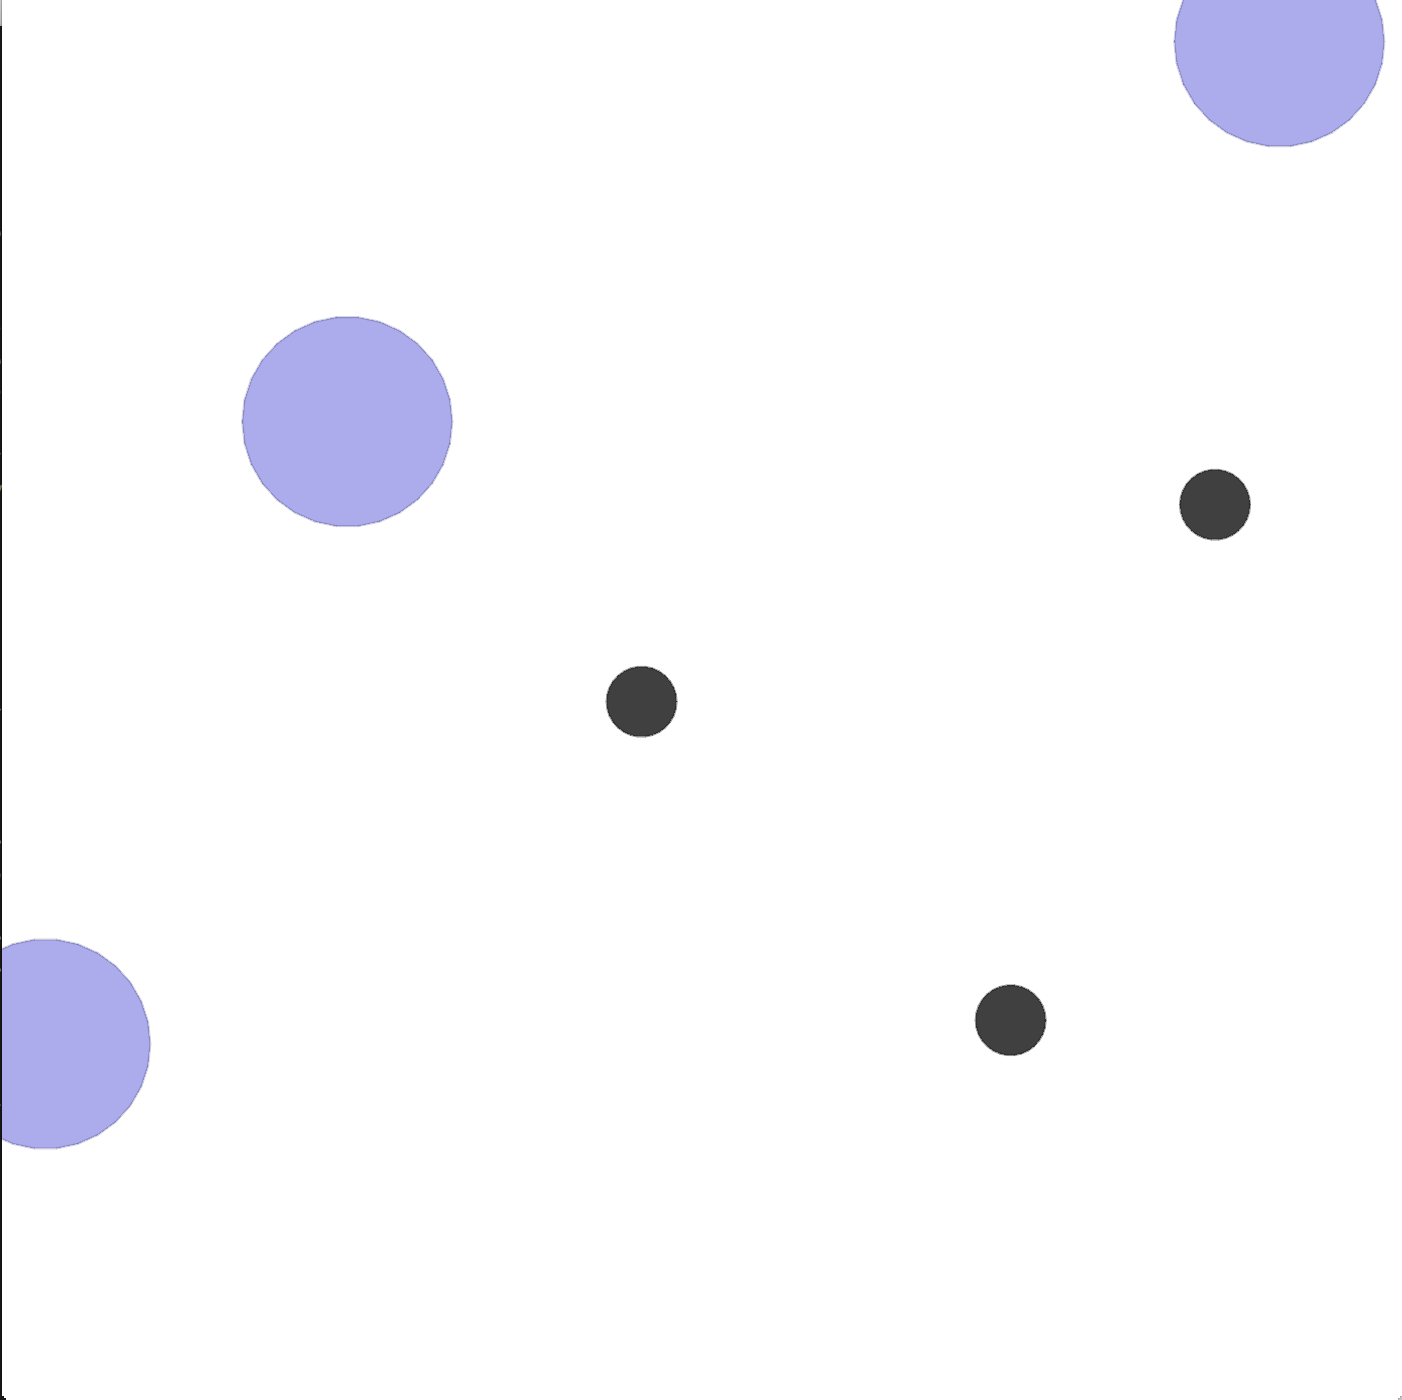
\includegraphics[scale=0.5]{env-image}
\end{center}
\caption{Cooperative navigation environment. Agents must learn to each navigate to a different landmark without colliding.}
\end{figure}

\subsection{Policy Gradient}
We implement a policy gradient algorithm as a baseline. Policy gradient algorithms seek to determine the optimal policy by directly adjusting the parameters $\theta$ of a policy $\pi_\theta$ in order to maximize the objective function $J*(\theta) = \mathbb{E}_{\pi_\theta}[R]$. We also implemented a baseline and advantage for the policy gradient. Letting $\hat{A} = R_t - b(s_t)$ be the advantage estimate at time t, we can write the gradient of the policy as:
$$\nabla_\theta J(\theta) = \mathbb{E}_{s,\pi_\theta}[\nabla_\theta log \pi_\theta(a|s)\hat{A}]$$
In the above equation, the expectation is taken over many sample trajectories through the environment using $\pi_\theta$. Policy gradient algorithms are already susceptible to  high variance, and executing them in a multi-agent environments only amplifies the problem. From a single agent's perspective not only does the world change as other agents move, but the policies other agents follow change as well. Additionally, individual agents might not always get the correct gradient signal as an agent could take a good action but if other agents took bad actions, leading to overall decrease in reward, the gradient for the agent taking the correct action could still be negative.

\subsection{MADDPG}

\begin{figure}
\begin{center}
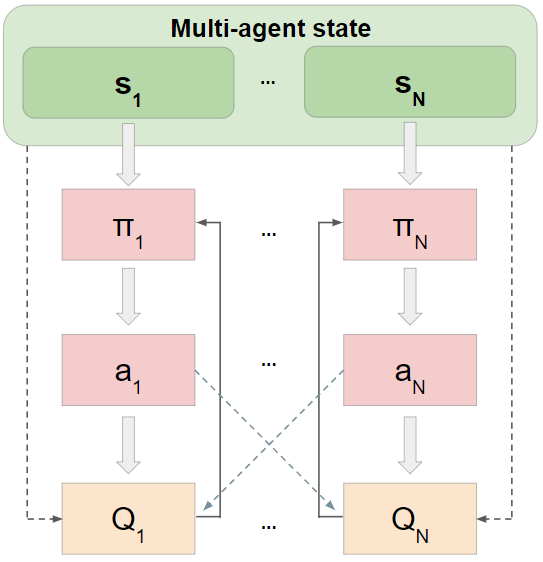
\includegraphics[scale=0.5]{maddpg-diagram}
\end{center}
\caption{MADDPG algorithm with centralized Q functions. As indicating by the dotted lines, note that the Q functions take the entire multi-agent state as an input in addition to the actions of all agents.}
\label{fig:diagram}
\end{figure}

We recreate MADDPG as our main algorithm for the cooperative navigation task ~\cite{maddpg}.  MADDPG takes DDPG and tailors it to multi-agent environmnnts, resulting in significantly better performance than single-agent methods. MADDPG trains separate policy networks for every agent, but uses a centralized action-value function that incorporates information across all agents to ensure a more stable learning process. 

Consider a game with $N$ agents, and let $\pi = \{\pi_1, ..., \pi_N\}$ be the associated set of agent policies that are parametrized by $\theta_1, ..., \theta_N$. Additionally let $s = \{s_1, ..., s_N\}$ represent the set of states observed by each agent. When using MADDPG to train agents, every agent additionally maintains a critic function that outputs a Q-value given the states and actions of all agents (see Figure \ref{fig:diagram}):
$$Q^\pi_i(s, a_1, ..., a_N)$$
Standard Q-learning techniques are used to update the critic function. Note that for the cooperative navigation environment that we run our experiments on, the Q-values will be the same for all agents as the reward for all agents is the same. However, this Q-function formulation where every agent learns its own $Q^\pi_i$ allows MADDPG to generalize to environments where agents have different reward functions (e.g. adversarial games).

During training, agents now have information not just about the locations of other agents, but about the actions they will take as well. Therefore, the environment is stationary for any agent as it does not depend on other agent policies:
$$P(s_i'|s_i, a_1, ..., a_N, \pi_1, ..., \pi_N) = P(s_i'|s_i, a_1, ..., a_N)$$
The policy network updates for an agent are determined by maximizing the agents centralized Q-values. The gradient update is similar to the update used in the policy gradient, except that it uses the centralized Q-value instead of only looking at the returns across trajectories:
$$\nabla_{\theta_i}J(\theta_i) = \mathbb{E}_{s, \pi_i}[\nabla_{\theta_i}log \pi_i(a_i|o_i)Q^{\pi}_i(x, a_1, ..., a_N)]$$
By incorporating the actions of all agents into the action-value function during training instead of only each individual agent, MADDPG produces better and more stable results than traditional policy gradient or Q-learning approaches. An additional advantage of using this extra information during training is that it we can implement and use experience replay as well. When training, we repeatedly sample from agent policy networks and store the result state transition in an experience replay buffer. Periodically, we update network parameters by sampling from the replay buffer and applying MADDPG to the sampled transitions.

During policy execution, agents only use their learned policy networks and therefore do not use any information about other agents; MADDPG is an enhancement to the training process while leaving the execution phase unchanged.

\subsection{More scalable MADDPG}
In addition to implementing MADDPG as described in the previous section, we further modify it to scale to better support large numbers of agents. The Q function described above increases linearly in input size as more agents are added to the scenario, as it has to take every agent's observation and action as an input. In order to reduce the additional computation time needed as $N$ grows, we modify MADDPG to only look at the $K$ nearest neighbors during training, where $K < N-1$. The mathematical formulation of the algorithm remains the same, but the inputs to $Q^\pi_i$ vary based on which agents are closest to $i$ at each timestep.

\subsection{Ornstein-Uhlenbeck action noise}
One of the exploration methods we have tried in our experiments, presented in the next section, is the Ornstein-Uhlenbeck (OU) noise process \cite{ou}. OU noise is a stochastic process that roughly models Brownian motion, and is also known as the correlated additive Gaussian action space noise. The idea behind using this process is that if the noise generated at a given time step is correlated to previous noise, it will tend to stay in the same direction for longer durations instead of immediately canceling itself out, which will consequently allow the agent to go towards the goal faster. So in the case of continuous actions it is better to have temporally correlated exploration that suit the dynamics to get smoother transitions. This noise process is popularly used with DDPG and we wanted to check if MADDPG can perform better with this exploration choice.

\section{Experiments and Results}
\subsection{Evaluation Metrics}

In order to evaluate the performance of our algorithms, every 250 training steps we do evaluation by running 40 episodes using the latest learned policies and calculate various metrics over them. Our primary evaluation metric for all experiments is average reward, which in this environment corresponds to the distance between agents and the target landmarks while also accounting for collisions that occur along the way. In addition to average reward, we also look at average distance between landmarks and agents, for more intuitive interpretation of the performance. Here we provide a detailed definition of average reward and average distance used in this paper, unless specified otherwise.

\textbf{Average reward.} Average reward is calculated by summing up rewards received from all agents, all timesteps within an episode, and then averaging across multiple episodes. Average rewards shown in plots are computed during dedicated evaluation runs whose data do not go into training set. The range of average reward is zero to negative infinity. 

\textbf{Average distance.} Average distance is the sum of distances between each agent and its closest landmark, across all agents and all timesteps within an episode, and then averaged across episodes.

Besides the metrics defined above, each experiment may additional context-specific evaluation metric, which will be defined for that experiment.


\subsection{Implementation details}

Table \ref{tab:basecase_parameters} lists the default hyperparameters used in our experiments. We use neural networks with a softmax activation at the final output layer to represent both the policy and Q networks.

\textbf{Episode Length.} The number of of actions every agent can take from the start state until the episode ends.

\textbf{Batch size.} The sequence of agent observations, actions, rewards and next observations used to train agents. We define the batch size in terms of episodes, so for a batch size of 50 episodes, we are actually using $50*25 = 1250$ timesteps at each training step.

\textbf{Timesteps per training batch.} This frequency defines how often we sample a training batch from the experience replay buffer (which stores $10^6$ timesteps) and update network parameters with it. At timesteps where we are not training we use the current agent policies to run episodes and obtain new training data to store in the replay buffer.

\textbf{Gamma.} It is the discount factor which models the future rewards as a fraction of the immediate rewards. It quantifies how much importance we give for future rewards.

\textbf{Learning rate.} Learning rate specifies the magnitude of step that is taken towards the solution. 

\textbf{Tau.} Affects how fast the target policy and Q networks update. 

\begin{table}[h!]
  \begin{center}
    
    \label{tab:basecase_parameters}
    \begin{tabular} {|l|l|} % <-- Changed to S here.
      \hline
      \textbf{Hyperparameter} & \textbf{Value} \\
      \hline
      \# of hidden layers & 2 \\
      \# of units per hidden layer & 128 \\
      Episode length (timesteps) & 25 \\
      Training batch size (in episodes) & 50 \\
      \# of training batches & 60,000 \\
			Timesteps per training batch & 100 \\
      Gamma ($\gamma$) & 0.95 \\
      Learning Rate ($\alpha$) & 0.01 \\
			Tau ($\tau$) & 0.01 \\
      \hline
    \end{tabular}
  \end{center}
	\caption{Default hyperparameters used for training MADDPG}
\end{table}

\subsection{Experiments}

\textbf{Baseline comparison.} As a baseline, we compare the performance of our policy gradient baseline and MADDPG with the baseline hyperparameters as given in Table \ref{tab:basecase_parameters} except with a batch size of 1024 episodes as used in \cite{maddpg}. As shown in Figures \ref{fig:MADDPGvsPG} and \ref{fig:MADDPGvsPG_distance}, the policy gradient approach has difficulties learning a good policy. It fails to improve while training and produces extremely noisy results. In contrast, MADDPG's performance steadily improves as training progresses and it exhibits much less variation in results, indicating that training is more stable. We believe MADDPG's performance comes from the fact that it uses a centralized critic function to allow agents to train themselves to make more accurate decisions given what other agents do as well.

\begin{figure}
\begin{center}
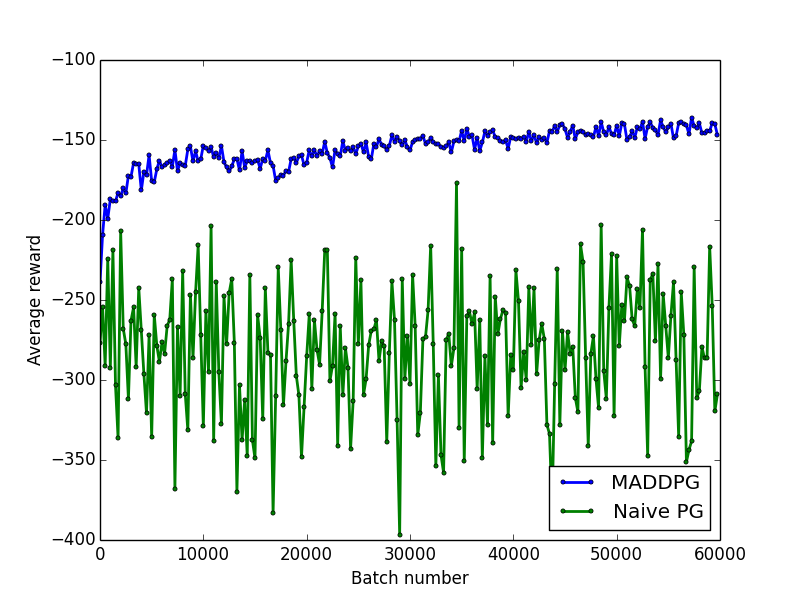
\includegraphics[scale=0.4]{MADDPGvsPG}
\end{center}
\caption{Average reward achieved by policy gradient algorithm and MADDPG algorithm.}
\label{fig:MADDPGvsPG}
\end{figure}

\begin{figure}
\begin{center}
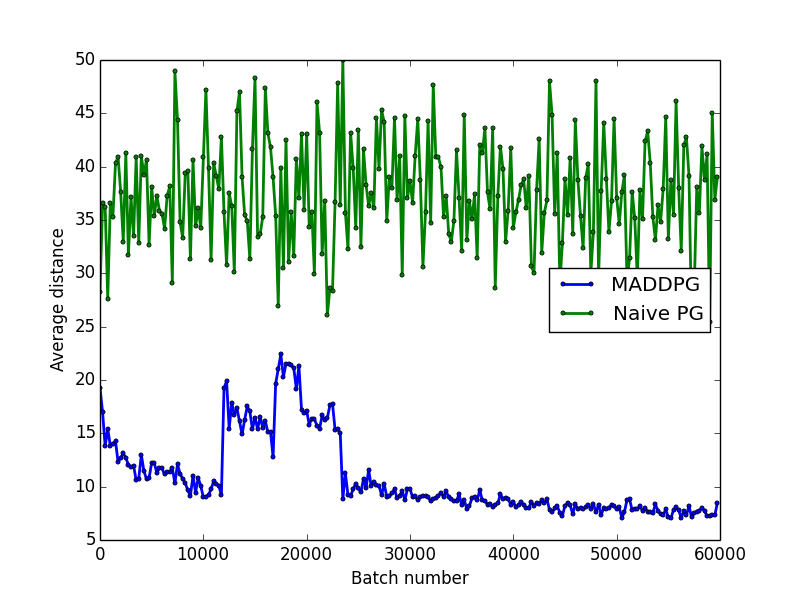
\includegraphics[scale=0.4]{MADDPGvsPG_distance}
\end{center}
\caption{Average distance from landmarks with Naive PG algorithm and MADDPG algorithm.}
\label{fig:MADDPGvsPG_distance}
\end{figure}

\textbf{Baseline comparison.} \textbf{TODO ONCE WE HAVE THE PLOT}

\textbf{Exploration strategies.} Next, we experimented experiment with 3 different methods of action exploration. First, we try re-implementing what Open AI does, which adds noise onto unnormalized policy network output, and then takes softmax to get the final action. We also try using Ornstein-Uhlenbeck process, with $\sigma = 0.3, \theta = 0.15$. Lastly, we experiment sampling from multivariate normal distribution with a trainable standard deviation. Figure \ref{fig:defaultVSouVSdist} shows the plot for average rewards with different action exploration strategies.

We found that applying noise to unnormalized policy network output outperforms other strategies. This finding corroborates the inference mentioned in \cite{plappert2017parameter} and can be extended to our experiments as well. The inference is that since the reward function is well-shaped, we do not need a lot of exploration for the cooperative navigation environment we have chosen. Therefore we use that as our default exploration when conducting other experiments. 

To further evaluate, we compare the Euclidean distance between the effective displacement as a result of pre-noise action versus post-noise action. The Euclidean distances are then averaged across every 100 steps (that is the training frequency) across all agents. Figure \ref{fig:action_exploration_range} and \ref{fig:action_exploration_std_dev} plot the range and standard deviation of the average Euclidean distances for the first 15000 batches.

\begin{figure}
\begin{center}
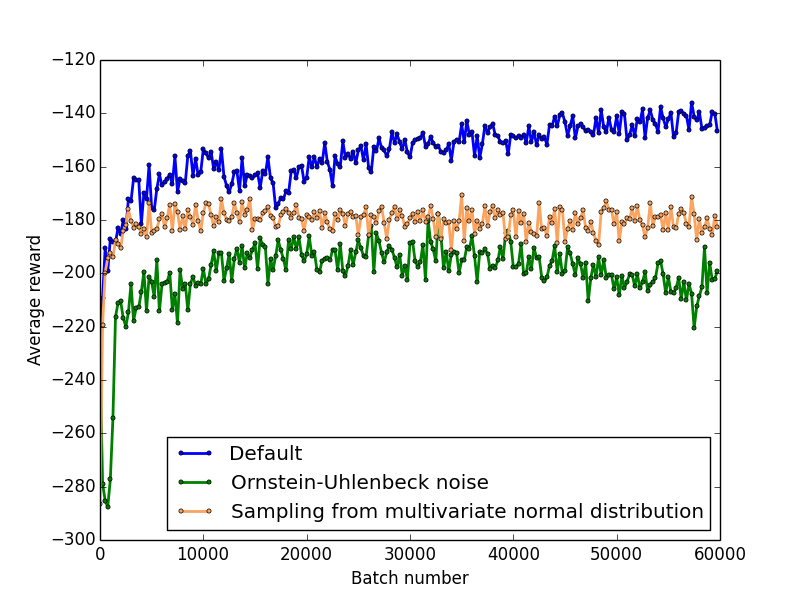
\includegraphics[scale=0.4]{defaultVSouVSdist}
\end{center}
\caption{Average reward gained by using different exploration strategies.}
\label{fig:defaultVSouVSdist}
\end{figure}


\begin{figure}
\begin{center}
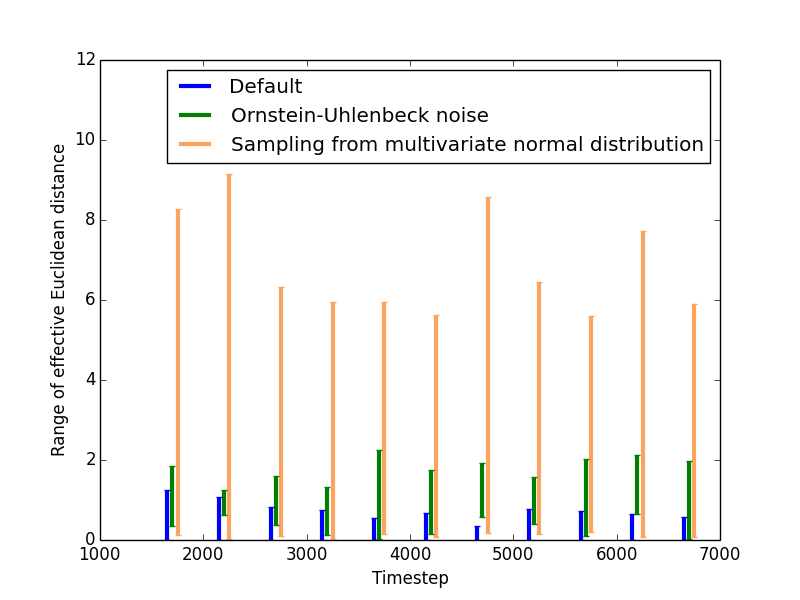
\includegraphics[scale=0.4]{action_exploration_range}
\end{center}
\caption{Range of effective euclidean distance for different exploration strategies.}
\label{fig:action_exploration_range}
\end{figure}

\begin{figure}
\begin{center}
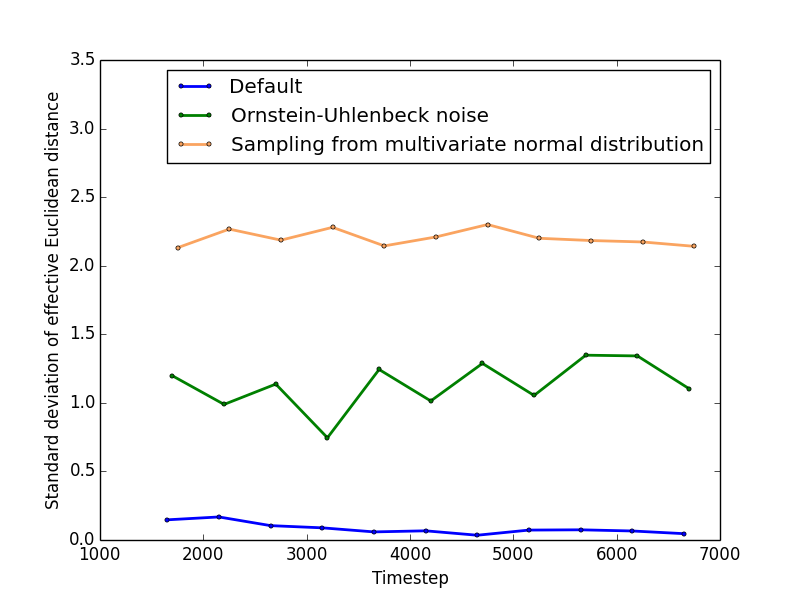
\includegraphics[scale=0.4]{action_exploration_std_dev}
\end{center}
\caption{Standard deviation of effective euclidean distance for different exploration strategies.}
\label{fig:action_exploration_std_dev}
\end{figure}

\begin{figure}
\begin{center}
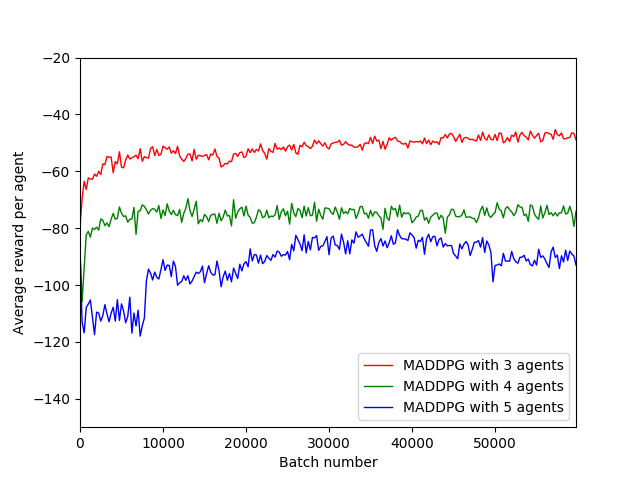
\includegraphics[scale=0.5]{maddpg_3,4,5agents.png}
\end{center}
\caption{Average reward gained by each agent in environment with different number of agents and landmarks}
\label{fig:avg_reward_multiple_agents}
\end{figure}

\textbf{Increased number of agents and landmarks.} Figure \ref{fig:avg_reward_multiple_agents} show the results from training different number of agents using MADDPG. For each result, the number of agents is equal to the number of landmarks. For smaller number of agents the average rewards increases with training whereas for even 1 or 2 more agents in the scenario, the training is not good enough. This can be attributed to the increased information from agents and increased complexity of environment due to more number of landmarks. Depending on the location of landmarks, the agents may or may not learn the policy for achieving the goal.   

\textbf{Changing network size.} We experimented with reducing the size of the neural network layers for the policy and Q networks to see the impact on training. We observed that the best achievable reward in a training run with 2-layer 64-unit networks (as opposed to the default of 2 layers with 128-unit networks) was around -175, which is noticeably lower than the -150 achieved with the default network size. This shows that the increased complexity of the neural networks do in fact help to define the right actions to take in the cooperative navigation task. 

\begin{figure}
\begin{center}
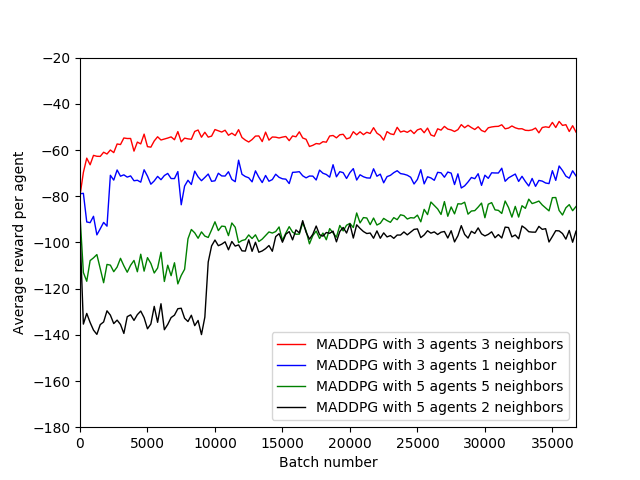
\includegraphics[scale=0.5]{MADDPG_different_neighbors.png}
\end{center}
\caption{Average reward gained by each agent with different number of neighboring agents information}
\label{fig:avg_reward_different_neighbors}
\end{figure}

\textbf{Scaling MADDPG to only use neighboring agents.} The input space of $Q$ grows linearly with the increase in the number of agents. This increases the memory requirements and the policies are learned very slowly. So we experimented with providing fewer neighbor information to the agent. The number of neighboring agent ($n$) info to be used is provided as a hyperparameter where $n < N$. Figure \ref{fig:avg_reward_different_neighbors} shows the performance of different agents using lesser number of neighbor info. This shows that the agents policies are not as good when using the information from all the neighbors.  

\section{Conclusion}

We introduced the problem of multi-agent reinforcement learning and show why traditional single-agent approaches are ineffective on these problems. We implemented a policy gradient method as a baseline and MADDPG, an algorithm designed for multi-agent scenarios, and applied them to the OpenAI cooperative navigation environment. We varied hyperparameters, changed the environment settings, applied different noise inputs and analysed the performance of MADDPG for different cases. 

We show that MADDPG clearly outperforms policy gradient approaches as it is able to steadily improvement performance over training batches while policy gradient fails to improve. 

\textbf{TODO - add more based on the experiments we put in} 


\section{Future Work}
We would like to try our approach on other multi-agent environments, in particular adversarial ones, to compare how MADDPG performs vs. policy gradients. It would also be interesting to explore how performance changes if agents are trained using different policies - e.g. in an adversarial game, what would happen if one set of agents were trained with MADDPG and a competing set were trained with policy gradients.

Our results from generalizing MADDPG to only look at $N$ nearest neighbors show that an agent might not even need to know about all other agents during training to achieve good results. We would like to further experiment with generalization, in particular by running against even larger numbers of agents.

Additionally, we would like to explore alternative forms of generalization. Instead of $Q^\pi_i$ looking at the $K$ nearest neighbors to agent $i$ for some fixed $K$, the Q-function could instead look at all neighbors within a particular distance to agent $i$. This way, the agents would have more information available to them when it is particularly important (the closer agents are to each other, the more likely it is to have a collision) while minimizing input space size when information about additional agents is less necessary.

\section*{Contributions}
Diana wrote the initial implementation of MADDPG, Shalini wrote our logging/plotting code, and Nitin wrote the initial implementation of the policy gradient baseline. All of us iterated on the code with bugfixes and enhancements and ran experiments using our implementations.

\bibliography{final}
\bibliographystyle{icml2018}

\end{document}

